\section{Path-Planning from Human Language}

% add outline page with current section highlighted.
\begin{frame}{Outline}{ $ \null $ }
	\tableofcontents[currentsection]
	%\tableofcontents[currentsection,currentsubsection]
\end{frame}

\subsection{Algorithm}

\begin{frame}{Language Understanding}{ Model Path-Planning from Human Language }

\begin{columns}
	\column{0.5\textwidth}
	\begin{figure}
		\centering
		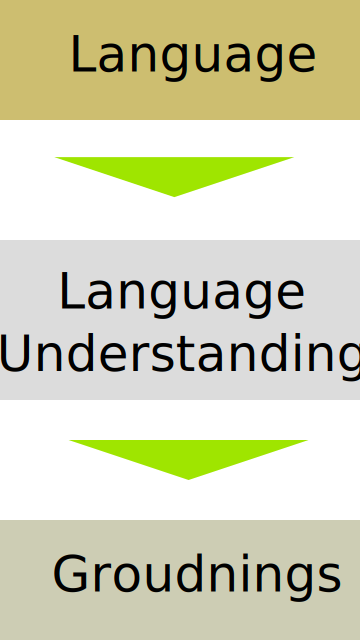
\includegraphics[width=.5\linewidth]{figure/language_understanding}
		\caption{Grounding process\footnotemark}
	\end{figure}	
	\column{0.5\textwidth}
	\begin{itemize}
	\item {\bf Phrases  $ \lambda $}

	\item {\bf Groundings $ \gamma $}
	\begin{itemize}
		\item actions
		\item landmarks / regions
		\item spatial relations
	\end{itemize}
	\end{itemize}
	
	\begin{block}{}
	\begin{equation}
	\nonumber
	\arg \max_{\gamma} P( \gamma \mid \lambda )
 	\end{equation}
 	\end{block}
 	
\end{columns}

\footnotetext[1]{\tiny {\it Tellex et al.} ``Understanding Natural Language Commands for Robotic Navigation and Mobile Manipulation.'' AAAI 2011. }

\end{frame}

\begin{frame}{Graphical Model}{ Model Path-Planning from Human Language }

\begin{columns}
\column{0.5\textwidth}
\begin{figure}
	\centering
	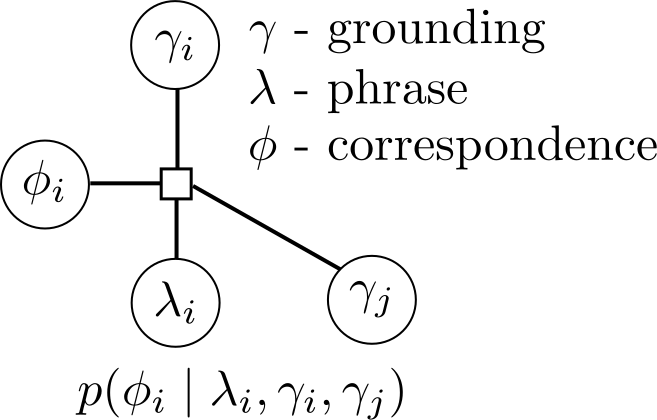
\includegraphics[width=.8\linewidth]{figure/factor_model}
\end{figure}
\column{0.5\textwidth}
\begin{itemize}
\item {\bf Correspondence $ \phi $}
\end{itemize}

\begin{block}{}
\begin{equation}
\nonumber
\arg \max_{\phi} P( \phi \mid \gamma , \lambda )
\end{equation}
\end{block}

\end{columns}

\end{frame}

\begin{frame}{Phrase Tree}{ Model Path-Planning from Human Language }

{\bf ``Move near the red box and the blue crate.''}

\begin{columns}
\column{0.5\textwidth}
\begin{figure}
	\centering
	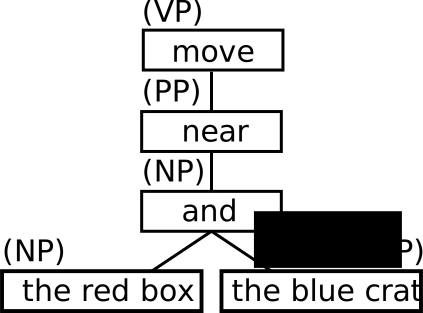
\includegraphics[width=.8\linewidth]{figure/phrase_structure2}
\end{figure}
\column{0.5\textwidth}
\begin{itemize}
\item A tree structure created by the grammar
\item Bottom-up dependencies
\end{itemize}
\end{columns}

\end{frame}

\begin{frame}{Graphical Model}{ Model Path-Planning from Human Language }

{\bf ``Move near the red box and the blue crate.''}

\begin{columns}
\column{0.5\textwidth}
\begin{figure}
	\centering
	\includegraphics[width=.9\linewidth]{figure/G3}
	\caption{ \tiny{ Howard et al. "A natural language planner interface for mobile manipulators." {\it IEEE International Conference on Robotics and Automation (ICRA) 2014.} } }
\end{figure}
\column{0.45\textwidth}
\begin{itemize}
\item Organizing factor models by the phrase tree
\end{itemize}
\end{columns}

\end{frame}

\begin{frame}{Distributed Correspondence Graph}{ Model Path-Planning from Human Language }
	
{\bf ``Move near the red box and the blue crate.''}
	
\begin{columns}
\column{0.5\textwidth}
\begin{figure}
	\centering
	\includegraphics[width=.9\linewidth]{figure/DCG}
	\caption{ \tiny{ Howard et al. "A natural language planner interface for mobile manipulators." {\it IEEE International Conference on Robotics and Automation (ICRA) 2014.} } }
\end{figure}
\column{0.45\textwidth}
\begin{itemize}
\item Train each factor model separately
\item Organize factor models into a graph model by the instruction for inference
\end{itemize}
\end{columns}

\end{frame}	

\begin{frame}{Groundings for Path-Planning}{ Model Path-Planning from Human Language } 

\begin{eqnarray}
\nonumber
\mbox{minimize: } & c(\sigma) = \int_{ \sigma } c(x) dx \\
\nonumber
\mbox{subject to: } & \sigma(0) = x_{init} \\
\nonumber
& \sigma(T) = x_{goal} \\
\nonumber
& H( \sigma(s) ) = 0 , s \in [0, T] 
\end{eqnarray}

\begin{columns}
\column{0.47\textwidth}
\begin{block}{Objective}
\begin{itemize}
\item shape of a cost function
\begin{itemize}
\item \textcolor{blue}{``avoiding ... ''}
\end{itemize}
\item types of cost functions
\begin{itemize}
\item \textcolor{blue}{``carefully ... ''}
\end{itemize}
\end{itemize}
\end{block}
\column{0.47\textwidth}
\begin{block}{Constraint}
\begin{itemize}
\item goal position / region
\begin{itemize}
\item \textcolor{blue}{``move to ... ''}
\end{itemize}
\item shapes of paths
\begin{itemize}
\item \textcolor{blue}{``by the left of ... ''}
\end{itemize}
\end{itemize}
\end{block}
\end{columns}

\end{frame}

\begin{frame}{Correspondence to the Cost Function}{ Model Path-Planning from Human Language }

{\bf Cost Function}	
	
\begin{columns}	
\column{0.3\textwidth}	
\begin{block}{World Model}
\begin{figure}
	\centering
	\includegraphics[width=.9\linewidth]{figure/world_model}
\end{figure}
\end{block}
\column{0.3\textwidth}
\begin{block}{Costmap}
\begin{figure}
	\centering
	\includegraphics[width=.9\linewidth]{figure/costmap}
\end{figure}
\end{block}
\column{0.3\textwidth}
\begin{block}{Path}
\begin{figure}
	\centering
	\includegraphics[width=.9\linewidth]{figure/costmap_path}
\end{figure}
\end{block}
\end{columns}

\begin{figure}
	\centering
	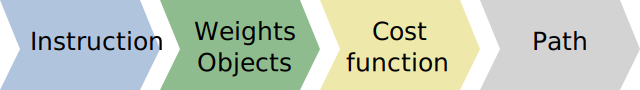
\includegraphics[width=.9\linewidth]{figure/cost_func_inference}
\end{figure}

\end{frame}

\begin{frame}{CDCG}{ Model Path-Planning from Human Language }

	\begin{itemize}
	\item {\bf Approximate the cost function by weighted sum of kernel functions}
	\begin{equation}
	\nonumber
	F( x \mid o_1 , \cdots , o_n ) = \sum_{i=1}^{n} w_i K( x \mid o_i )
	\end{equation}
	\item {\bf Ground the sentence to a cost function}
	\begin{equation}
	\nonumber
	\arg \max_{ F \in \bm{F} } p( F \mid \Lambda , \Upsilon )
	\end{equation}
	\item {\bf Continuous correspondence variables}
	\begin{equation}
	\nonumber
	\arg \max_{ w_i } \prod p'( w_i \mid \gamma_i , \lambda_i, \Gamma_{c_i} , \Upsilon )
	\end{equation}	
	\end{itemize}

\end{frame}

\begin{frame}{CDCG}{ Model Path-Planning from Human Language }
	
{\bf A mixed structure of continuous and discrete correspondence variables}
	
\begin{figure}
	\centering
	\includegraphics[width=.6\linewidth]{figure/DCG_network_structure}
\end{figure}
	
\end{frame}

\begin{frame}{HDCG}{ Model Path-Planning from Human Language }
	
	{\bf Homotopy}
	
	\begin{columns}	
	\column{0.3\textwidth}	
	\begin{block}{World Model}
	\begin{figure}
		\centering
		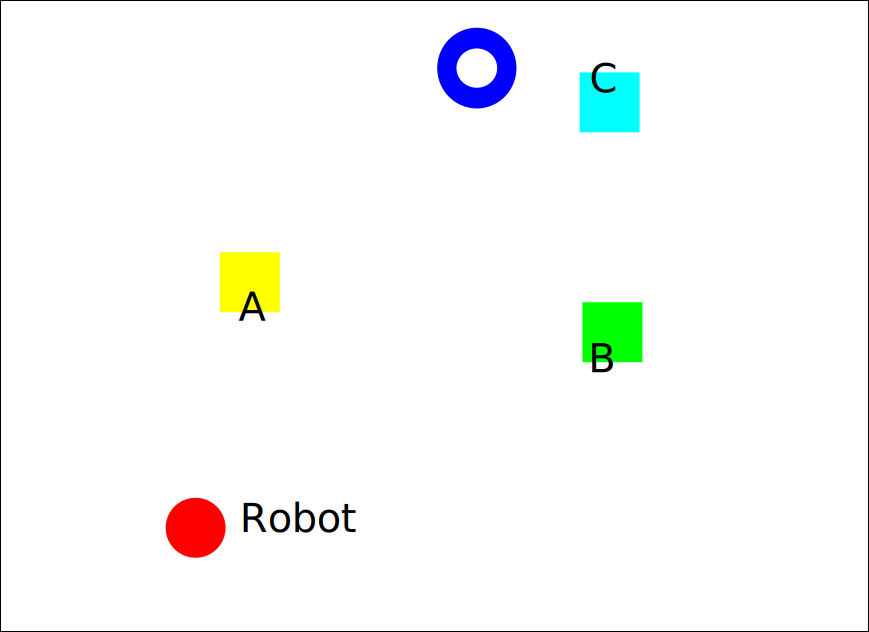
\includegraphics[width=.9\linewidth]{figure/homotopy/example_a}
	\end{figure}
	\end{block}
	\column{0.3\textwidth}
	\begin{block}{Costmap}
	\begin{figure}
		\centering
		\includegraphics[width=.9\linewidth]{figure/homotopy/example_a_decomp}
	\end{figure}
	\end{block}
	\column{0.3\textwidth}
	\begin{block}{Path}
	\begin{figure}
		\centering
		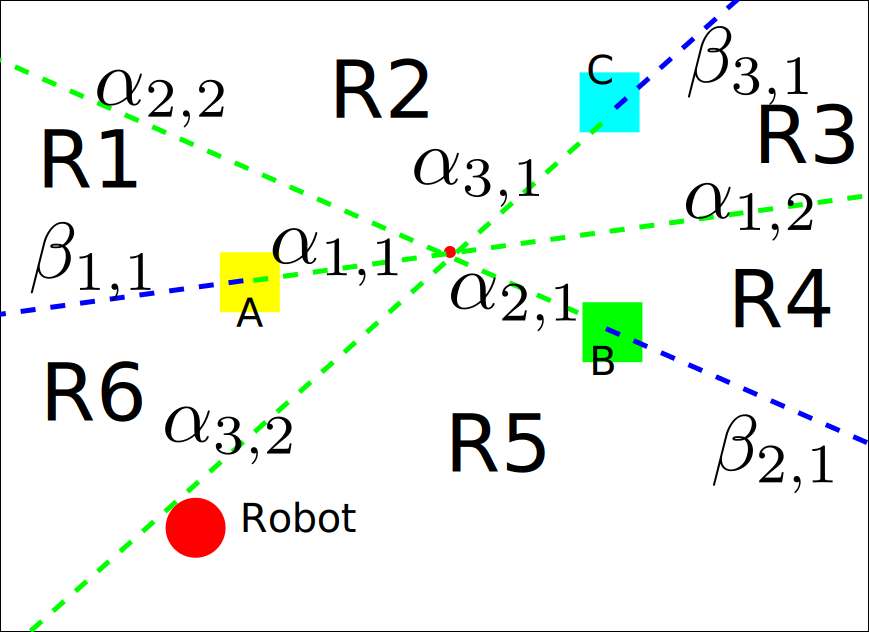
\includegraphics[width=.9\linewidth]{figure/homotopy/example_a_path}
	\end{figure}
	\end{block}
	\end{columns}
	
	\begin{figure}
		\centering
		\includegraphics[width=.9\linewidth]{figure/homotopy_inference}
	\end{figure}

\end{frame}

\begin{frame}{HDCG}{ Model Path-Planning from Human Language }

\begin{block}{Spatial relation function\footnotemark}
\begin{itemize}
\item $ R = ${\sc InBetween }$ ( \{ o_1 , o_2 \} ) $
\item $ R = ${\sc LeftOf }$ ( \{ o \} ) $ and $ R = ${\sc RightOf }$ ( \{ o \} ) $
\item $ \bar{R} = ${\sc Avoid}$ ( \{ o \} )  $
\item $ R = ${\sc Around }$ ( \{ o \} ) $
\end{itemize}
\end{block}

\begin{block}{Groundings correspond to an instruction}
\begin{itemize}
\item Objects / landmarks $ o $
\item Spatial relation functions
\end{itemize}
\end{block}

\begin{block}{Construct topological constraints}
\begin{itemize}
\item define eligible homotopy classes
\item optimal paths of eligible homotopy classes
\end{itemize}
\end{block}

\footnotetext[2]{\tiny {\it Oh et al.} ``Toward Mobile Robots Reasoning Like Humans.'' AAAI 2015.}

\end{frame}

\subsection{Validation}

\begin{frame}{Validation - Data Collection}{ Model Path-Planning from Human Language }

\begin{block}{Annotating paths}
Amazon Mechanic Turk
\end{block}

\begin{columns}	
	\column{0.6\textwidth}	
	\begin{figure}
		\centering
		\includegraphics[width=.9\linewidth]{figure/annotation_task}
	\end{figure}
	\column{0.3\textwidth}	
	\begin{figure}
		\centering
		\includegraphics[width=\linewidth]{figure/example_xml}
	\end{figure}
\end{columns}
\begin{block}{Generating example dataset}
Associate groundings with phrases
\end{block}

\end{frame}

\begin{frame}{Validation - Performance}{ Model Path-Planning from Human Language }

\begin{block}{Tranining a model with examples dataset}
Evaluate how the model fits the example dataset
\end{block}

\begin{block}{Inference using with the trained model}
Find groundings from a language instruction
\end{block}

\end{frame}




